\sectionframe{Datenquellen}
\subsection{Excel-Tabellen}
\begin{frame}
 \frametitle{Aufbau einer \texttt{SheetConnection}}
 Der Objekt-Datentyp \texttt{SheetConnection} stellt Verbindungen zu Excel-Tabellen dar (nur unter MS Windows).
 \begin{block}{Erstellen einer \texttt{SheetConnection}}
  \ttfamily
  SheetConnection \textsf{\slshape Name}("\textsf{\slshape Pfad der Tabelle}");
 \end{block}
 \begin{block}{Mögliche Datentypen für Einlesen und Schreiben}
  \begin{itemize}
   \item nulldimensionale Datentypen, d.h. einfache Variablen. Auslesen einer einzelnen Zelle.
   \item eindimensionale Datentypen, d.h. Sets und einfache Arrays. Auslesen einer Zeile oder Spalte.
   \item zweidimensionale Datentypen, d.h. zweidimensionale Arrays. Auslesen einer Zellenmatrix.
  \end{itemize}
 \end{block}
\end{frame}

\begin{frame}
 \frametitle{Lesen und Schreiben mit absoluter Zelladressierung}
 \begin{block}{Lesen mit absoluter Zelladressierung}
  \ttfamily
  \textsf{\slshape Variablename} from SheetRead(\textsf{\slshape SheetConnection-Name}, "\textsf{\slshape Tabellenname}!\textsf{\slshape Startzelle}:\textsf{\slshape Endzelle}")
 \end{block}
 \begin{block}{Schreiben mit absoluter Zelladressierung}
  \ttfamily
  \textsf{\slshape Variablename} to SheetWrite(\textsf{\slshape SheetConnection-Name}, "\textsf{\slshape Tabllenname}!\textsf{\slshape Startzelle}:\textsf{\slshape Endzelle}")
 \end{block}
\end{frame}

\begin{frame}[fragile]
 \frametitle{In Beispiel "`Vindoo Support"'}
 \begin{block}{Excel-Tabelle für Beispiel "`Vindo Support"'}
  \centering
  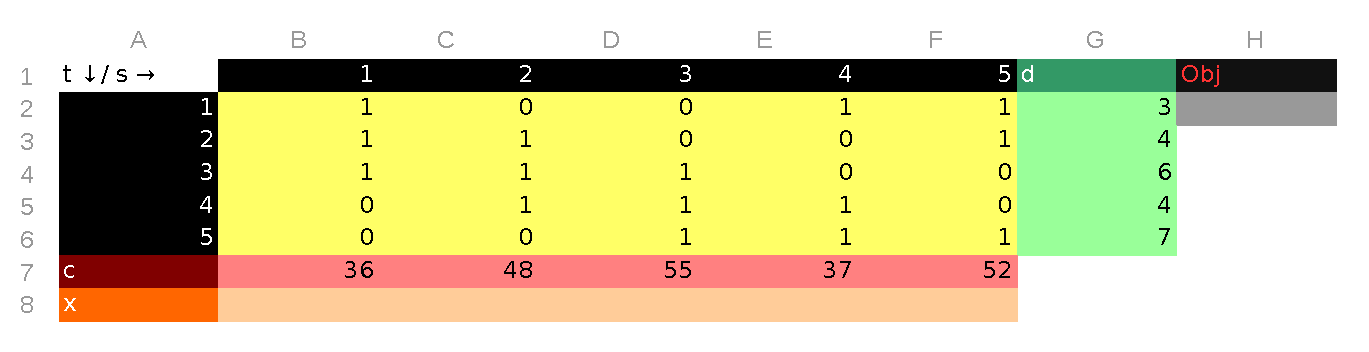
\includegraphics[width=.9\linewidth]{Bilder/CyclicStaffingData}
 \end{block}
 \begin{block}{Auszüge aus der Datendatei}
\begin{lstlisting}[language=opldata,numbers=none,basicstyle=\ttfamily\scriptsize]
// SheetConnection
SheetConnection sheet("CyclicStaffingProblem.xls");
\end{lstlisting}\vspace{-2\baselineskip}
\begin{lstlisting}[language=opldata,numbers=none,basicstyle=\ttfamily\scriptsize]
// Indexmengen
T from SheetRead(sheet, "Data!B1:F1");
\end{lstlisting}\vspace{-2\baselineskip}
\begin{lstlisting}[language=opldata,numbers=none,basicstyle=\ttfamily\scriptsize]
//Parameter
d from SheetRead(sheet, "Data!G2:G6");
\end{lstlisting}\vspace{-2\baselineskip}
\begin{lstlisting}[language=opldata,numbers=none,basicstyle=\ttfamily\scriptsize]
//Entscheidungsvariablen
x to SheetWrite(sheet, "Data!B8:F8");
\end{lstlisting}
 \end{block}
\end{frame}

\begin{frame}
 \frametitle{Lesen und Schreiben mit Namensbereichen}
 MS Excel ermöglicht es einzelnen Zellbereichen Namen zu geben.
 \begin{block}{Lesen mit Namensbereichen}
  \ttfamily
  \textsf{\slshape Variablename} from SheetRead(\textsf{\slshape SheetConnection-Name}, "\textsf{\slshape Bereichsname}")
 \end{block}
 \begin{block}{Schreiben mit Namensbereichen}
  \ttfamily
  \textsf{\slshape Variablename} to SheetWrite(\textsf{\slshape SheetConnection-Name}, "\textsf{\slshape Bereichsname}")
 \end{block}
\end{frame}

\begin{frame}[fragile]
 \frametitle{In Beispiel "`Vindoo Support"'}
 \begin{block}{Excel-Tabelle für Beispiel "`Vindo Support"'}
  \begin{center}
   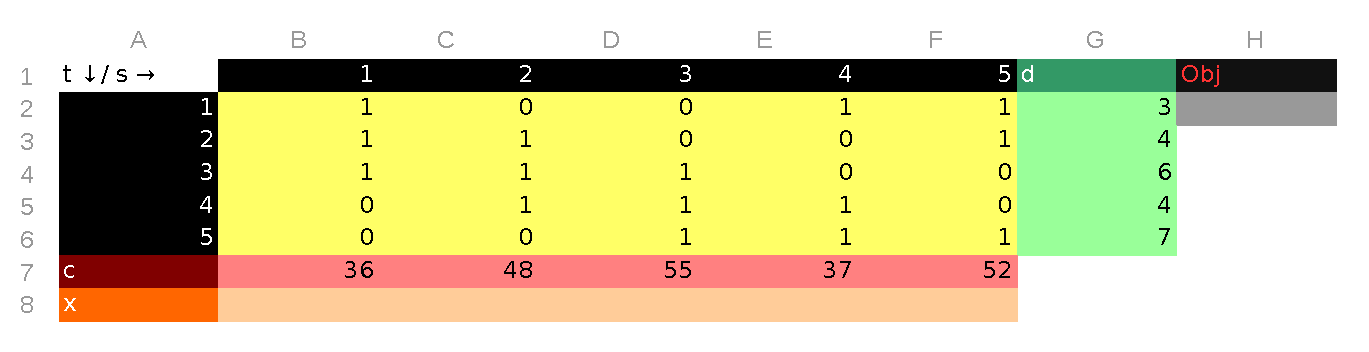
\includegraphics[width=.9\linewidth]{Bilder/CyclicStaffingData}
  \end{center}\vspace{-1\baselineskip}
  Der gelbe Bereiche heiße "`\texttt{ParamA}"'
 \end{block}
 \begin{block}{Auszüge aus der Datendatei}
\begin{lstlisting}[language=opldata,numbers=none,basicstyle=\ttfamily\scriptsize]
// SheetConnection
SheetConnection sheet("CyclicStaffingProblem.xls");
\end{lstlisting}\vspace{-2\baselineskip}
\begin{lstlisting}[language=opldata,numbers=none,basicstyle=\ttfamily\scriptsize]
//Parameter
a from SheetRead(sheet, "ParamA");
\end{lstlisting}
 \end{block}
\end{frame}

\subsection{Datenbanken}
\begin{frame}
 \frametitle{Aufbau einer \texttt{DBConnection}}
 Der Objekt-Datentyp \texttt{DBConnection} stellt Verbindungen zu einer Datenbank dar.
 \begin{block}{Erstellen einer \texttt{DBConnection}}
  \ttfamily
  DBConnection \textsf{\slshape Name}("\textsf{\slshape Schnittstelle}", "\textsf{\slshape Verbindungs-String}");
 \end{block}
 \begin{block}{Unterstützte Datenbank-Schnittstellen}
  \begin{itemize}
   \item DB2
   \item Oracle (Version 10 und 11)
   \item OLE DB (MS SQL Server)
   \item ODBC (u.a. für MS Access)
  \end{itemize}
 \end{block}
\end{frame}

\begin{frame}
 \frametitle{Beispiel-Datenbank: \texttt{CyclicStaffingProblem}}
 \begin{table}[htbp]\tiny
 \begin{tabularx}{\linewidth}{XX}
  \begin{minipage}{\linewidth}
   \begin{subtable}[b]{\linewidth}
     \centering
     \begin{tabular}{ccc}
      \toprule
      \ttfamily s 
\includegraphics[width=1em]{Bilder/Key} & \ttfamily t 
\includegraphics[width=1em]{Bilder/Key} & \ttfamily a \\
      \midrule
      \arrayrulecolor{gray!30}
      1 & 1 & 1 \\
      1 & 2 & 1 \\
      1 & 3 & 1 \\
      1 & 4 & 0 \\
      1 & 5 & 0 \\
      \midrule
      2 & 1 & 0 \\
      2 & 2 & 1 \\
      2 & 3 & 1 \\
      2 & 4 & 1 \\
      2 & 5 & 0 \\
      \midrule
      3 & 1 & 0 \\
      3 & 2 & 0 \\
      3 & 3 & 1 \\
      3 & 4 & 1 \\
      3 & 5 & 1 \\
      \midrule
      4 & 1 & 1 \\
      4 & 2 & 0 \\
      4 & 3 & 0 \\
      4 & 4 & 1 \\
      4 & 5 & 1 \\
      \midrule
      5 & 1 & 1 \\
      5 & 2 & 1 \\
      5 & 3 & 0 \\
      5 & 4 & 0 \\
      5 & 5 & 1 \\
      \arrayrulecolor{black}
      \bottomrule
     \end{tabular}
    \caption{Tabelle \texttt{A}}
    \end{subtable}
  \end{minipage}
  &
  \begin{minipage}{\linewidth}
    \begin{subtable}[b]{\linewidth}
     \centering
     \begin{tabular}{cc}
      \toprule
      \ttfamily ind 
\includegraphics[width=1em]{Bilder/Key} & \ttfamily d \\
      \midrule
      1 & 2 \\
      2 & 4 \\
      3 & 6 \\
      4 & 4 \\
      5 & 7 \\
      \bottomrule
     \end{tabular}
    \caption{Tabelle \texttt{T}}
    \end{subtable}
    \bigskip\bigskip
    
    \begin{subtable}[b]{\linewidth}
     \centering
     \begin{tabular}{ccc}
      \toprule
      \ttfamily ind 
\includegraphics[width=1em]{Bilder/Key} & \ttfamily c & \ttfamily x \\
      \midrule
      1 & 36 \\
      2 & 48 \\
      3 & 55 \\
      4 & 37 \\
      5 & 52 \\
      \bottomrule
     \end{tabular}
    \caption{Tabelle \texttt{S}}
    \end{subtable}
  \end{minipage}
 \end{tabularx}
\end{table}
\end{frame}

\begin{frame}[fragile]
 \frametitle{Einlesen von Array-Daten}
 Die Beispiel-Datenbank \texttt{CyclicStaffingProblem} sei über eine ODBC-Schnittstelle verbunden. Der User "`\texttt{user}"' mit dem Passwort "`\texttt{password}"' hat die nötige Zugangsberechtigung.
 \begin{block}{Auszüge aus der Datendatei}
\begin{lstlisting}[language=opldata,numbers=none,basicstyle=\ttfamily\scriptsize]
// DBConnection
DBConnection 
  db("odbc", "CyclicStaffingProblem/user/password");
\end{lstlisting}\vspace{-2\baselineskip}
\begin{lstlisting}[language=opldata,numbers=none,basicstyle=\ttfamily\scriptsize]
// Indexmengen
T from DBRead (db, "SELECT ind from T");
\end{lstlisting}\vspace{-2\baselineskip}
\begin{lstlisting}[language=opldata,numbers=none,basicstyle=\ttfamily\scriptsize]
// Parameter
c from DBRead(db, "SELECT ind,c from S");
a from DBRead(db, "SELECT t,s,a from A");
\end{lstlisting}
 \end{block}
\end{frame}

\begin{frame}[fragile]
 \frametitle{Einlesen und Schreiben von Tupel-Daten}
 \begin{block}{Auszüge aus der Modelldatei}
\begin{lstlisting}[language=opl,numbers=none,basicstyle=\ttfamily\scriptsize]
//Tuple
tuple shift{
  int ind;
  float c;
}
tuple result{<
  int x;
  int ind;
}  
\end{lstlisting}\vspace{-2\baselineskip}
\begin{lstlisting}[language=opl,numbers=none,basicstyle=\ttfamily\scriptsize]
//Postprocessing
{result} r = {<x[s],s.ind>|s in S};
\end{lstlisting}
 \end{block}\vspace{-2\baselineskip}
 \begin{block}{Auszüge aus der Datendatei}
\begin{lstlisting}[language=opldata,numbers=none,basicstyle=\ttfamily\scriptsize]
//Indexmengen
S from DBRead(db, "SELECT ind,c from S");
\end{lstlisting}\vspace{-2\baselineskip}
\begin{lstlisting}[language=opldata,numbers=none,basicstyle=\ttfamily\scriptsize]
//Entscheidungsvariablen
r to DBUpdate(db, "UPDATE S SET x=? WHERE ind=?");
\end{lstlisting}
 \end{block}
\end{frame}

